\documentclass[twoside]{article}
\setlength{\oddsidemargin}{0.25 in}
\setlength{\evensidemargin}{-0.25 in}
\setlength{\topmargin}{-0.6 in}
\setlength{\textwidth}{6.5 in}
\setlength{\textheight}{8.5 in}
\setlength{\headsep}{0.75 in}
\setlength{\parindent}{0 in}
\setlength{\parskip}{0.1 in}

\usepackage{graphicx}
\usepackage{url}

%
% The following commands sets up the lecnum (lecture number)
% counter and make various numbering schemes work relative
% to the lecture number.
%
\newcounter{lecnum}
\renewcommand{\thepage}{\thelecnum-\arabic{page}}
\renewcommand{\thesection}{\thelecnum.\arabic{section}}
\renewcommand{\theequation}{\thelecnum.\arabic{equation}}
\renewcommand{\thefigure}{\thelecnum.\arabic{figure}}
\renewcommand{\thetable}{\thelecnum.\arabic{table}}
\newcommand{\dnl}{\mbox{}\par}

%
% The following macro is used to generate the header.
%
\newcommand{\lecture}[4]{
  \pagestyle{myheadings}
  \thispagestyle{plain}
  \newpage
  \setcounter{lecnum}{#1}
  \setcounter{page}{1}
  \noindent
  \begin{center}
  \framebox{
     \vbox{\vspace{2mm}
   \hbox to 6.28in { {\bf CMPSCI~630~~~Systems
                       \hfill Spring 2017 } }
      \vspace{4mm}
      \hbox to 6.28in { {\Large \hfill Lecture #1  \hfill} }
%       \hbox to 6.28in { {\Large \hfill Lecture #1: #2  \hfill} }
      \vspace{2mm}
      \hbox to 6.28in { {\it Lecturer: #3 \hfill Scribe: #4} }
     \vspace{2mm}}
  }
  \end{center}
  \markboth{Lecture #1: #2}{Lecture #1: #2}
  \vspace*{4mm}
}

%
% Convention for citations is authors' initials followed by the year.
% For example, to cite a paper by Leighton and Maggs you would type
% \cite{LM89}, and to cite a paper by Strassen you would type \cite{S69}.
% (To avoid bibliography problems, for now we redefine the \cite command.)
%
\renewcommand{\cite}[1]{[#1]}

% \input{epsf}

%Use this command for a figure; it puts a figure in wherever you want it.
%usage: \fig{NUMBER}{FIGURE-SIZE}{CAPTION}{FILENAME}
\newcommand{\fig}[4]{
           \vspace{0.2 in}
           \setlength{\epsfxsize}{#2}
           \centerline{\epsfbox{#4}}
           \begin{center}
           Figure \thelecnum.#1:~#3
           \end{center}
   }

% Use these for theorems, lemmas, proofs, etc.
\newtheorem{theorem}{Theorem}[lecnum]
\newtheorem{lemma}[theorem]{Lemma}
\newtheorem{proposition}[theorem]{Proposition}
\newtheorem{claim}[theorem]{Claim}
\newtheorem{corollary}[theorem]{Corollary}
\newtheorem{definition}[theorem]{Definition}
\newenvironment{proof}{{\bf Proof:}}{\hfill\rule{2mm}{2mm}}

% Some useful equation alignment commands, borrowed from TeX
\makeatletter
\def\eqalign#1{\,\vcenter{\openup\jot\m@th
 \ialign{\strut\hfil$\displaystyle{##}$&$\displaystyle{{}##}$\hfil
     \crcr#1\crcr}}\,}
\def\eqalignno#1{\displ@y \tabskip\@centering
 \halign to\displaywidth{\hfil$\displaystyle{##}$\tabskip\z@skip
   &$\displaystyle{{}##}$\hfil\tabskip\@centering
   &\llap{$##$}\tabskip\z@skip\crcr
   #1\crcr}}
\def\leqalignno#1{\displ@y \tabskip\@centering
 \halign to\displaywidth{\hfil$\displaystyle{##}$\tabskip\z@skip
   &$\displaystyle{{}##}$\hfil\tabskip\@centering
   &\kern-\displaywidth\rlap{$##$}\tabskip\displaywidth\crcr
   #1\crcr}}
\makeatother

% **** IF YOU WANT TO DEFINE ADDITIONAL MACROS FOR YOURSELF, PUT THEM HERE:



% Some general latex examples and examples making use of the
% macros follow.

\begin{document}

%FILL IN THE RIGHT INFO.
%\lecture{**LECTURE-NUMBER**}{**DATE**}{**LECTURER**}{**SCRIBE**}
\lecture{9}{March 3rd}{Emery Berger}{Lurdh Pradeep Reddy Ambati, Karthik A., Vikram Pawar}

\section{OS Kernel}

A kernel is indispensable and therefore the most important part of an operating system. However, there are different design principles governing developing of a kernel. On the one end of the spectrum, there is the Monolithic kernel architecture and at the other end is the microkernel architecture.

\begin{figure}[h!]
\centering
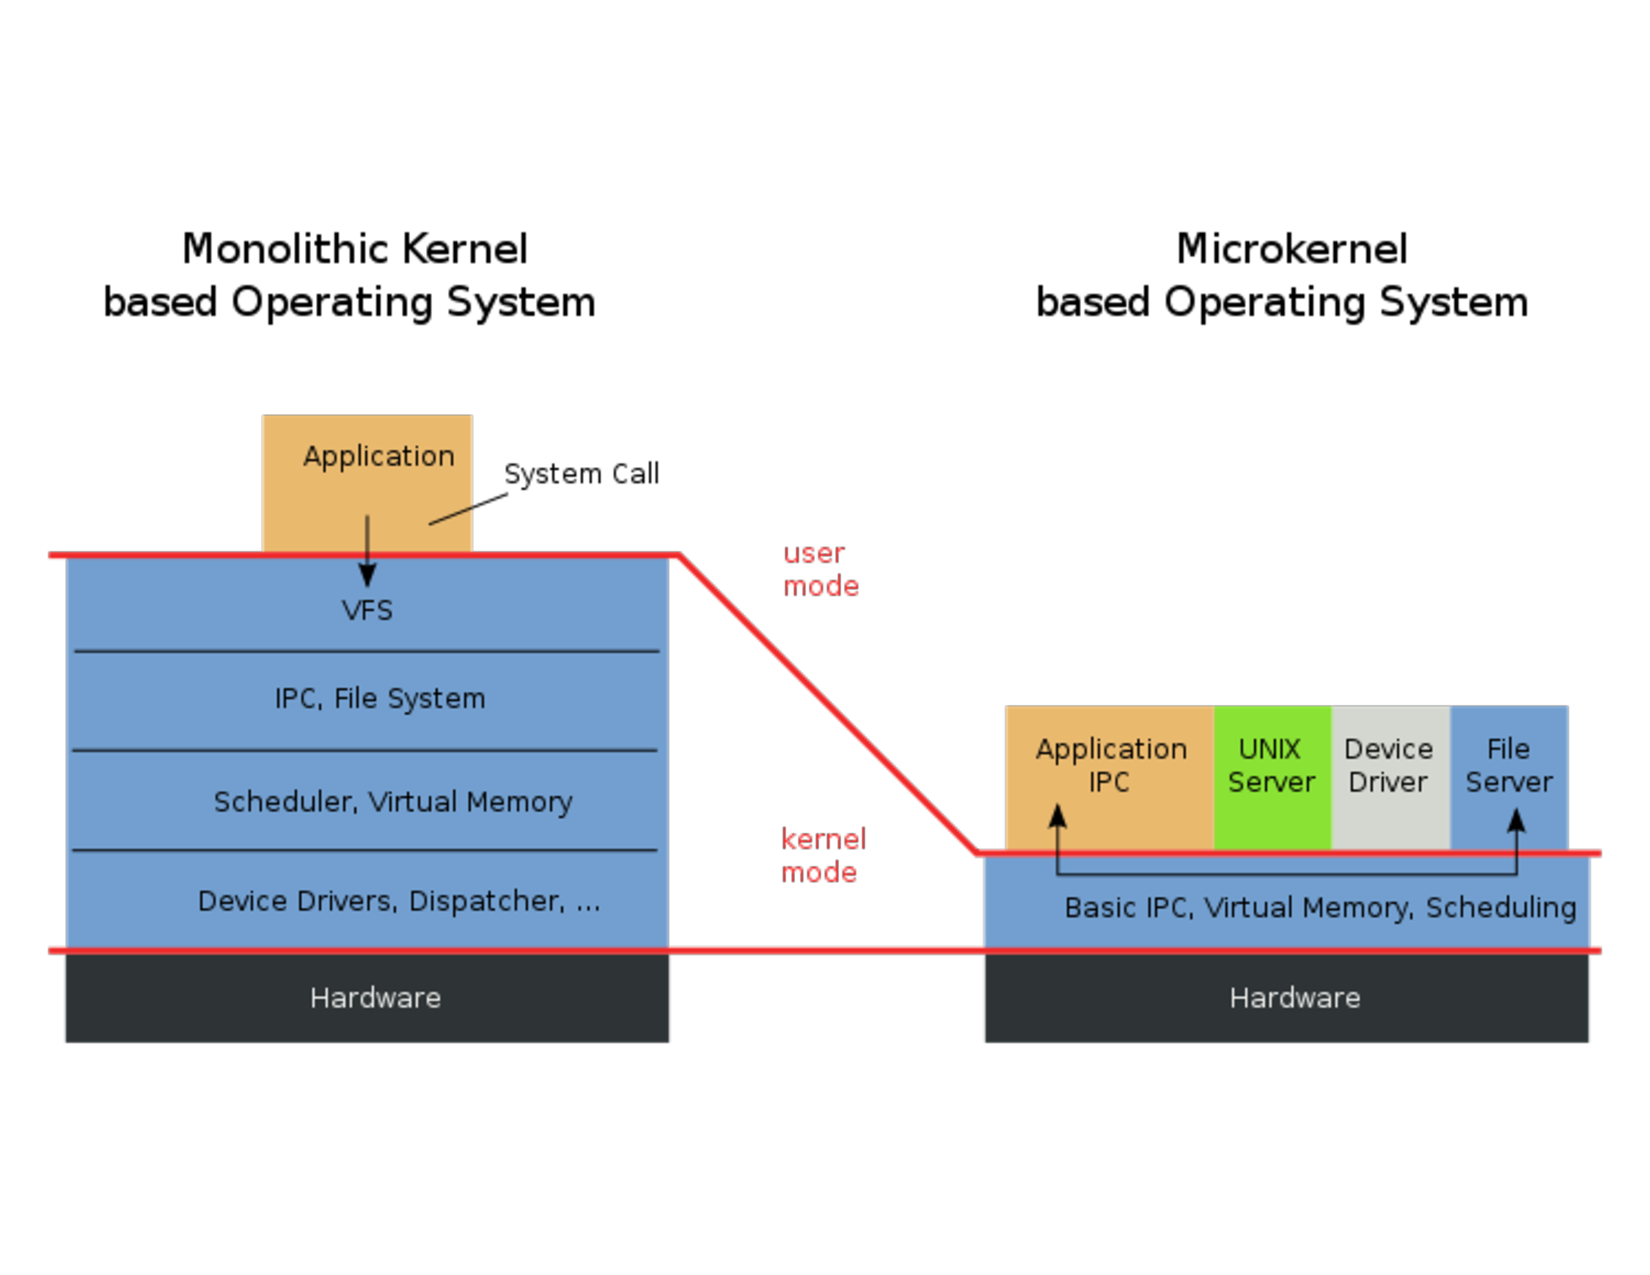
\includegraphics[width=0.4\linewidth]{kernel.pdf}
\caption{Monolithic kernel v/s micro kernel}
\label{fig:kernel_types}
\end{figure}

\subsection{ Monolithic Kernel}

A Monolithic kernel is an OS architecture where the entire operating system (which includes the device drivers, file system, and the application IPC) is working in kernel space. Monolithic kernels are able to dynamically load (and unload) executable modules at runtime. 

Examples of operating systems that use a monolithic kernel are - Linux, Solaris,  Microsoft Windows etc

 It is faster than micro kernel, but it is less secure as device driver can crash the kernel, and is bulky.

\subsection{Micro kernel}

In microkernels, the kernel is broken down into separate processes, known as servers. Some of the servers run in kernel space and some run in user-space. All servers are kept separate and run in different address spaces. Servers invoke "services" from each other by sending messages via IPC (Interprocess Communication). This separation has the advantage that if one server fails, other servers can still work efficiently. 

Examples of operating systems that use a microkernel are - QNX, Integrity, PikeOS, Symbian, L4Linux, Singularity, K42, Mac OS X, HURD, Minix, and Coyotos.

It is slower than monolithic kernel, but it is crash resistant (device drivers), smaller in size and adding a new service is simple as it does not involve recompiling entire kernel as opposed to early versions of monolithic kernels.

\section{User land}

User level application runs in "user land", which runs in the least privileged mode, where as the kernel runs in the most privileged mode. User land takes advantage of the way that the kernel smooths over minor hardware differences, presenting the same API to all programs. The kernel is usually interrupt-driven, either software interrupts (system calls) or hardware interrupts (disk drives, network cards, hardware timers). System calls from the user land to kernel pass through kernel boundary and during this process TLB are flushed, processor is switched from user mode to kernel mode and can potentially take 100-200 cycles for this transition. 

\section{Principle of least privilege}

The principle of least privilege (also known as the principle of minimal privilege or the principle of least authority) requires that in a particular abstraction layer of a computing environment, every module (such as a process, a user, or a program, depending on the subject) must be able to access only the information and resources that are necessary for its legitimate purpose.

Device drivers in monolithic kernel violate as they reside in kernel and they can access anything in kernel. (can see the physical memory and can access the other processes as well.)


\section{Layered approach for system design - "THE" multiprogramming system }

When multiple modules of a system have multiple interfaces, the number of possible interactions between them grows exponentially. This also means that it becomes less possible to test or mathematically prove the program correctness of all possible combinations of interactions. Instead, if we restrict the design to take a layered approach - where each layer can only be invoked by the layer immediately above it and each layer can only call methods of the layer below it - the number of possible interactions is reduced drastically. 

\begin{figure}[h!]
\centering
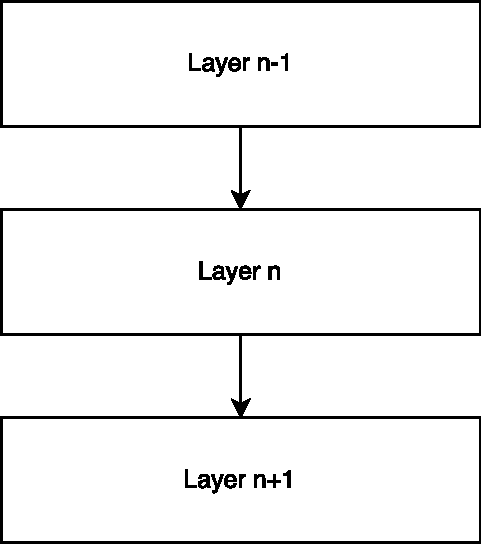
\includegraphics[width=0.2\linewidth]{layers.pdf}
\caption{Layered approach for system design}
\label{fig:layers}
\end{figure}

This advantage was used by Dijkstra in the design of "THE" multiprogramming system. To prove the correctness of the entire system, the correctness of each layer can be proved by only considering the layer above it and below it using techniques like Predicate Transformer (due to Dijkstra) and Hoare's triples (due to Tony Hoare).

\section{Mixins}

Mixin is an object oriented programming concept that can be used to implement layer based approach easily. Classes can be arranged in the form of layers to form Mixin Layers. A Mixin is usually a parameterized class and the parameter becomes the parent class. Multiple Mixin classes can be composed to form a system using layered design.

\section{The UNIX Operating System}

UNIX was developed by a small team comprising Ken Thompson, Dennis Ritchie and others at Bell Labs in the 1970s. The operating system borrowed advanced developed in Multics, which was a mega-project that failed due to its size and complexity. The team decided to make a lightweight and easy-to-use replacement for Multics that could be used by programmers at Bell Labs. 

\subsection{Everything is a file}
Unix included the brilliant design decision "everything is a file" - which meant that input-output devices, system information, text files and directories were all treated as byte-streams exposed through a file interface. 

\subsection{Pipes}
Unix implemented pipes, which allow the user to string together the inputs and outputs of multiple processes with a single command. This allows the user to execute a complex operation using a group of simple ones. The disadvantage of piping is that it starts up multiple processes and copies data from one process to another using inter-process-communication. This is less efficient than executing a single process.



\end{document}
